%%%%%%%%%%%%%%%%%%%%%%%%%%%%%%%%%%%%%%%%%%%%%%%%%%%%%%%%%%%%%%%%%%%%%%
% Overleaf (WriteLaTeX) Example: Molecular Chemistry Presentation
%
% Source: http://www.overleaf.com
%
% In these slides we show how Overleaf can be used with standard 
% chemistry packages to easily create professional presentations.
% 
% Feel free to distribute this example, but please keep the referral
% to overleaf.com
% 
%%%%%%%%%%%%%%%%%%%%%%%%%%%%%%%%%%%%%%%%%%%%%%%%%%%%%%%%%%%%%%%%%%%%%%

\documentclass{beamer}

\mode<presentation>
{
  \usetheme{Madrid}       % or try default, Darmstadt, Warsaw, ...
  \usecolortheme{default} % or try albatross, beaver, crane, ...
  \usefonttheme{default}    % or try default, structurebold, ...
  \setbeamertemplate{navigation symbols}{}
  \setbeamertemplate{caption}[numbered]
} 

\usepackage[english]{babel}
\usepackage[utf8x]{inputenc}
\usepackage{chemfig}
\usepackage[version=3]{mhchem}

\usepackage{hyperref}
  \hypersetup{colorlinks=true}
  \hypersetup{urlcolor=blue}
  \hypersetup{linkcolor = .}
\usepackage{xcolor}
\usepackage{siunitx}
  \sisetup{separate-uncertainty = true}
\usepackage{physics}
\usepackage[font=small,labelfont=bf]{caption}
\usepackage{subcaption}
\usepackage[en-GB]{datetime2}
\usepackage{feynmp}
\DeclareGraphicsRule{*}{mps}{*}{}

\usepackage{scalerel}
\newcommand{\mylbrace}[2]{\vspace{#2pt}\hspace{6pt}\scaleleftright[\dimexpr5pt+#1\dimexpr0.06pt]{\lbrace}{\rule[\dimexpr2pt-#1\dimexpr0.5pt]{-4pt}{#1pt}}{.}}
\newcommand{\myrbrace}[2]{\vspace{#2pt}\scaleleftright[\dimexpr5pt+#1\dimexpr0.06pt]{.}{\rule[\dimexpr2pt-#1\dimexpr0.5pt]{-4pt}{#1pt}}{\rbrace}\hspace{6pt}}

% Here's where the presentation starts, with the info for the title slide
\title[BESIII Oxford]{BESIII Oxford Group Meeting}
\author{Martin Tat}
\institute{Oxford LHCb}
\date{\today}

\titlegraphic{
\includegraphics[width = 5cm, height = 3.8cm]{lhcb.jpg}\hspace{1cm}~%
              
\includegraphics[width = 5cm, height = 3.8cm]{bes3.jpg}}

\begin{document}

\begin{frame}
  \titlepage
\end{frame}

% These three lines create an automatically generated table of contents.
%\begin{frame}{Outline}
%  \tableofcontents
%\end{frame}

\section{Intorduction}
\begin{frame}{Introduction}
  \begin{itemize}
    \setlength\itemsep{2em}
    \item{Double tagged $D\to K^+K^-\pi^+\pi^-$ events}
    \item{Previously: Fit $\Delta E$ in double tagged events}
    \begin{itemize}
      \item{Fixed to single tagged events, much better fit!}
    \end{itemize}
    \item{Fit to $m_\text{BC}$ of single tags to get ST yield}
    \item{Got TopoAna and MC truth matching working $\implies$ to study backgrounds}
  \end{itemize}
\end{frame}

\section{Double tag fit}
\begin{frame}{Double tag $\Delta E$ fit}
  \begin{figure}
    \centering
    \begin{subfigure}{0.4\textwidth}
      \centering
      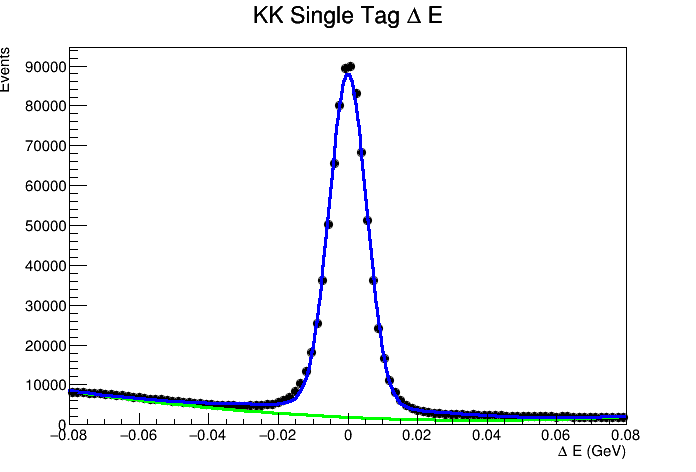
\includegraphics[width=\textwidth]{KKDeltaE.png}
      \caption{$\Delta E$, $KK$}
    \end{subfigure}%
    \begin{subfigure}{0.4\textwidth}
      \centering
      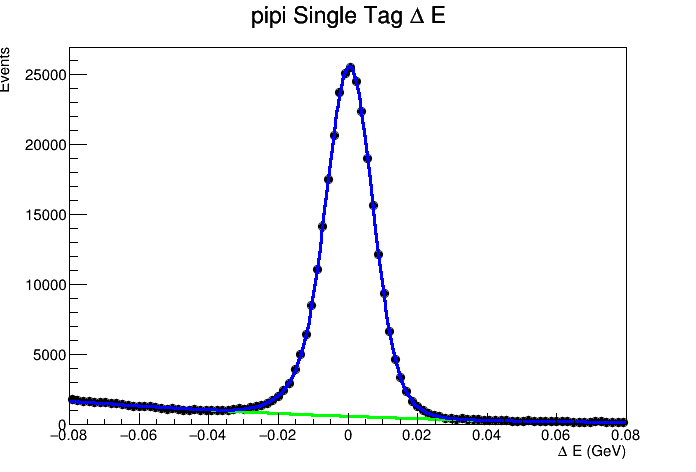
\includegraphics[width=\textwidth]{pipiDeltaE.png}
      \caption{$\Delta E$, $\pi\pi$}
    \end{subfigure}
    \begin{subfigure}{0.4\textwidth}
      \centering
      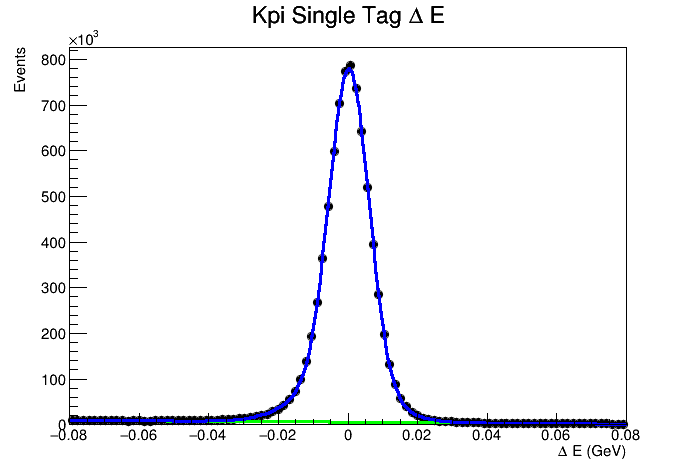
\includegraphics[width=\textwidth]{KpiDeltaE.png}
      \caption{$\Delta E$, $K\pi$}
    \end{subfigure}%
    \begin{subfigure}{0.4\textwidth}
      \centering
      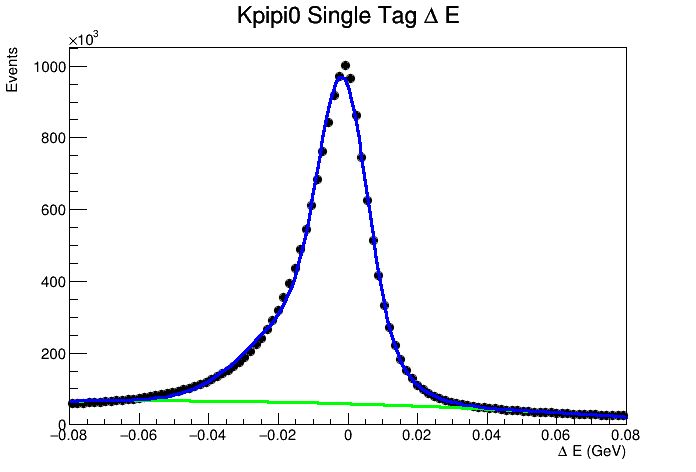
\includegraphics[width=\textwidth]{Kpipi0DeltaE.png}
      \caption{$\Delta E$, $K\pi\pi^0$}
    \end{subfigure}
  \end{figure}
\end{frame}

\begin{frame}{Double tag $\Delta E$ fit}
  \begin{figure}
    \centering
    \begin{subfigure}{0.4\textwidth}
      \centering
      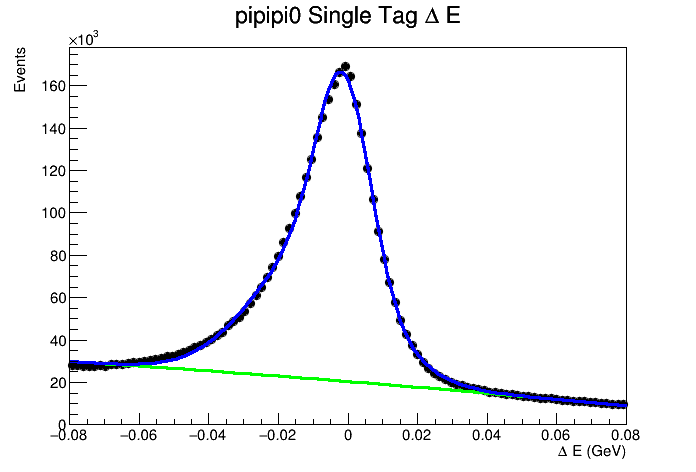
\includegraphics[width=\textwidth]{pipipi0DeltaE.png}
      \caption{$\Delta E$, $\pi\pi\pi^0$}
    \end{subfigure}%=
    \begin{subfigure}{0.4\textwidth}
      \centering
      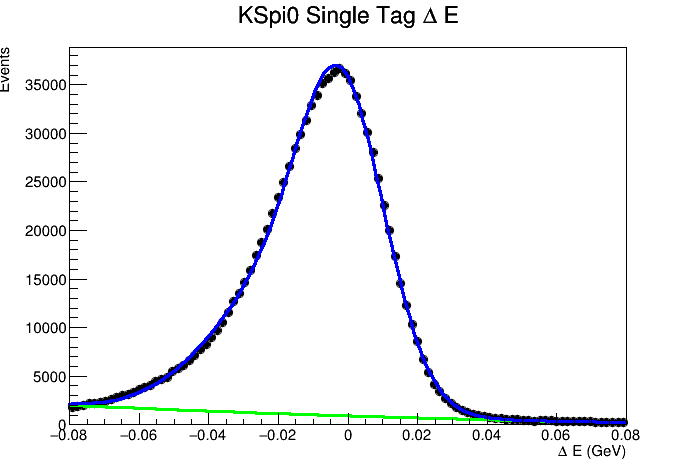
\includegraphics[width=\textwidth]{KSpi0DeltaE.png}
      \caption{$\Delta E$, $K_S\pi^0$}
    \end{subfigure}
    \begin{subfigure}{0.4\textwidth}
      \centering
      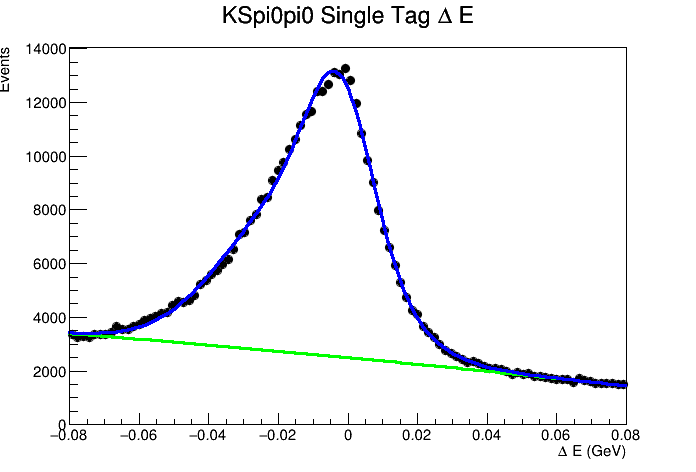
\includegraphics[width=\textwidth]{KSpi0pi0DeltaE.png}
      \caption{$\Delta E$, $K_S\pi^0\pi^0$}
    \end{subfigure}%
    \begin{subfigure}{0.4\textwidth}
      \centering
      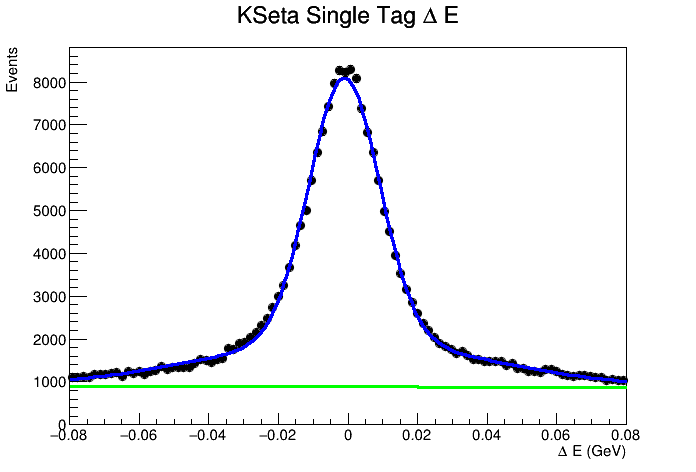
\includegraphics[width=\textwidth]{KSetaDeltaE.png}
      \caption{$\Delta E$, $K_S\eta$}
    \end{subfigure}
  \end{figure}
\end{frame}

\begin{frame}{Double tag $\Delta E$ fit}
  \begin{figure}
    \centering
    \begin{subfigure}{0.4\textwidth}
      \centering
      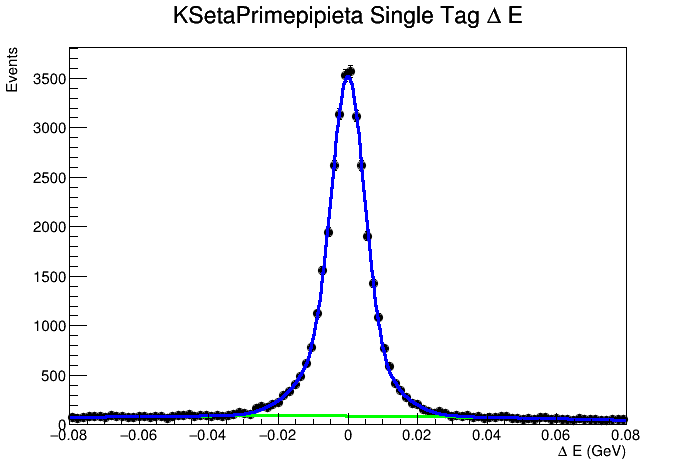
\includegraphics[width=\textwidth]{KSetaPrimepipietaDeltaE.png}
      \caption{$\Delta E$, $K_S\eta'(\pi\pi\eta)$}
    \end{subfigure}%
    \begin{subfigure}{0.4\textwidth}
      \centering
      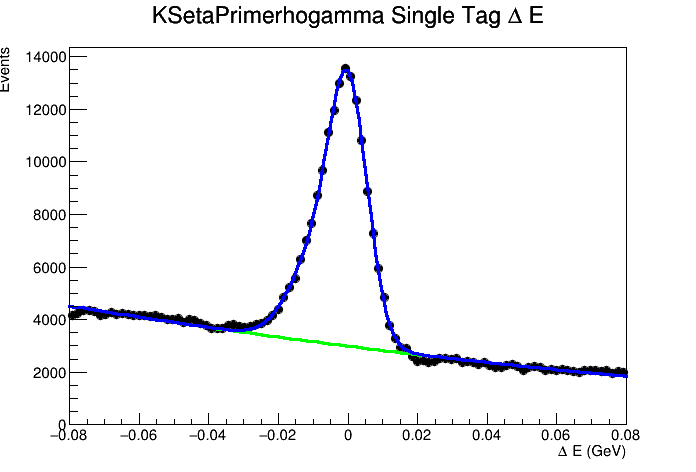
\includegraphics[width=\textwidth]{KSetaPrimerhogammaDeltaE.png}
      \caption{$\Delta E$, $K_S\eta'(\pi\pi\gamma)$}
    \end{subfigure}
    \begin{subfigure}{0.4\textwidth}
      \centering
      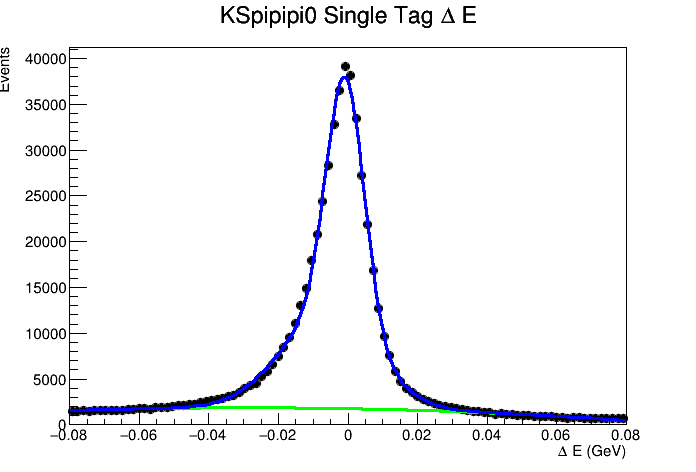
\includegraphics[width=\textwidth]{KSpipipi0DeltaE.png}
      \caption{$\Delta E$, $K\pi\pi\pi^0$}
    \end{subfigure}
  \end{figure}
\end{frame}

\begin{frame}{Double tag $\Delta E$ fit}
  \begin{figure}
    \centering
    \begin{subfigure}{0.4\textwidth}
      \centering
      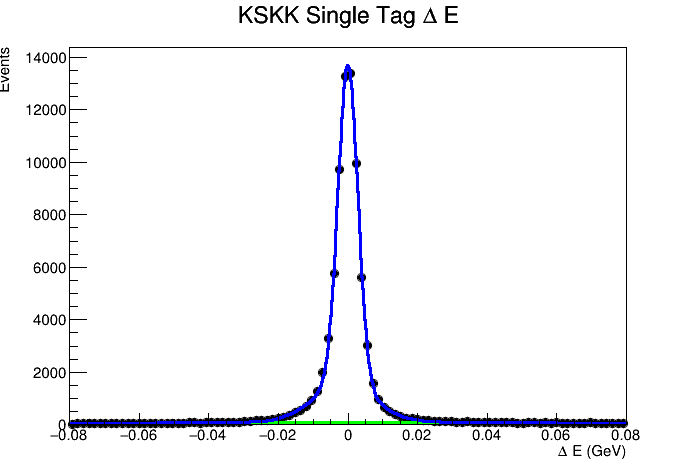
\includegraphics[width=\textwidth]{KSKKDeltaE.png}
      \caption{$\Delta E$, $K_SKK$}
    \end{subfigure}%
    \begin{subfigure}{0.4\textwidth}
      \centering
      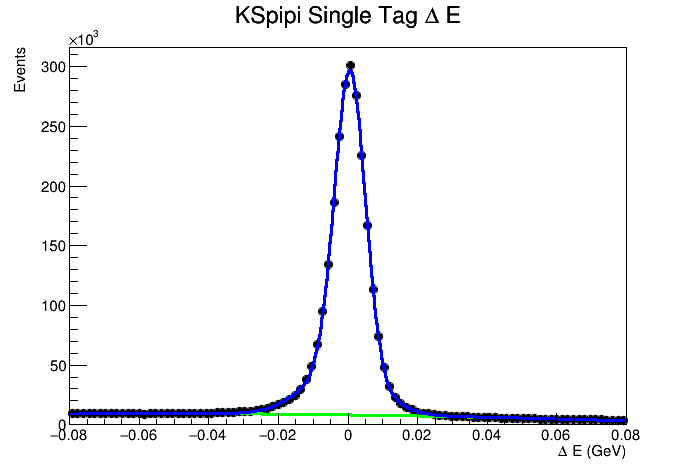
\includegraphics[width=\textwidth]{KSpipiDeltaE.png}
      \caption{$\Delta E$, $K_S\pi\pi$}
    \end{subfigure}
    \begin{subfigure}{0.4\textwidth}
      \centering
      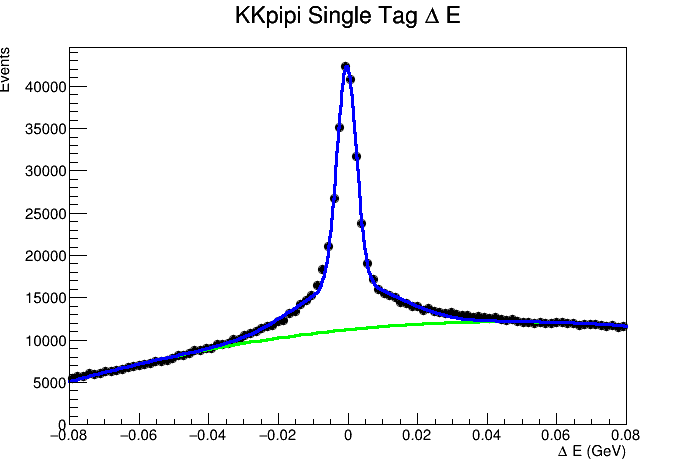
\includegraphics[width=\textwidth]{KKpipiDeltaE.png}
      \caption{$\Delta E$, $KK\pi\pi$}
    \end{subfigure}
  \end{figure}
\end{frame}

\begin{frame}{Single tag $m_\text{BC}$ fit}
  \begin{figure}
    \centering
    \begin{subfigure}{0.5\textwidth}
      \centering
      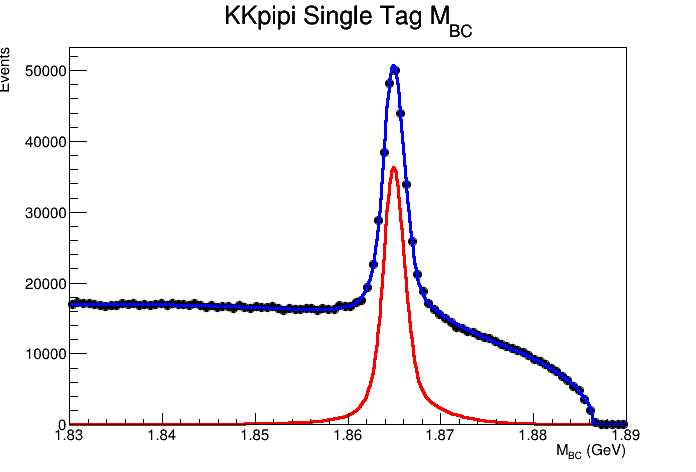
\includegraphics[width=\textwidth]{KKpipiMBCFit.png}
      \caption{$m_\text{BC}$, $KK\pi\pi$}
    \end{subfigure}%
    \begin{subfigure}{0.5\textwidth}
      \centering
      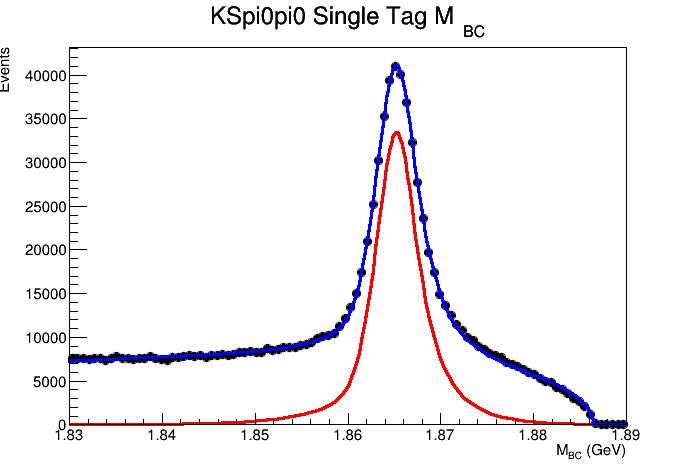
\includegraphics[width=\textwidth]{KSpi0pi0MBCFit.png}
      \caption{$m_\text{BC}$, $K_S\pi^0\pi^0$}
    \end{subfigure}
  \end{figure}
  Question: MC samples for signal shape?
\end{frame}

\section{Backgrounds}
\begin{frame}{Backgrounds}
  \begin{itemize}
    \setlength\itemsep{2em}
    \item{MC truth matching: Check for mis-ID and combinatorial}
    \item{TopoAna: Check peaking backgrounds}
    \begin{itemize}
      \item{Had to remove intermediate resonances from decay tree}
    \end{itemize}
  \end{itemize}
\end{frame}

\begin{frame}{Example: $\pi\pi$ single tag}
  \begin{figure}
    \centering
    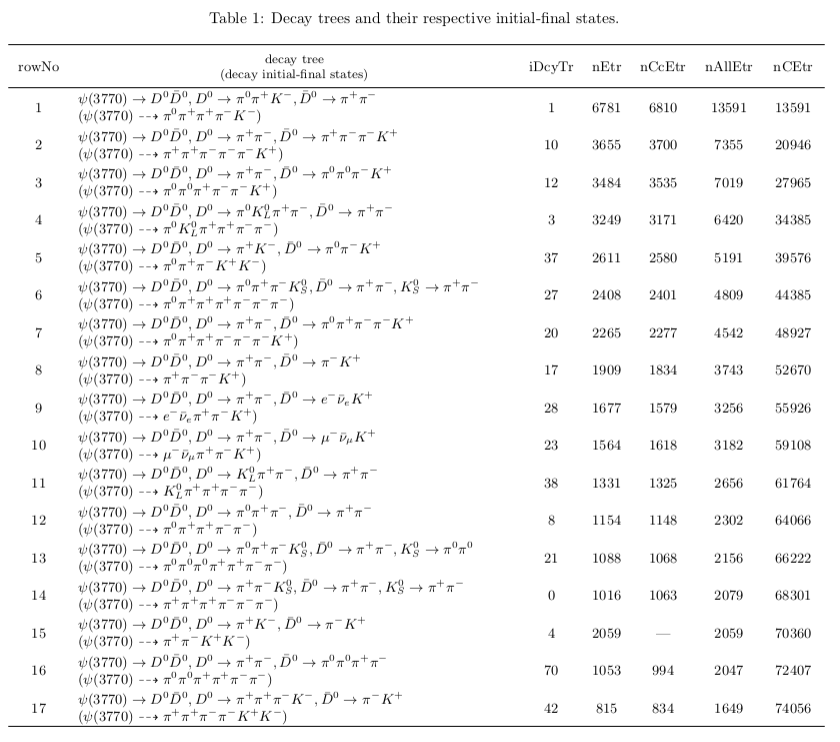
\includegraphics[width=0.7\textwidth]{pipiDecayTree.png}
  \end{figure}
\end{frame}

\begin{frame}{Example: $\pi\pi$ single tag}
  \begin{figure}
    \centering
    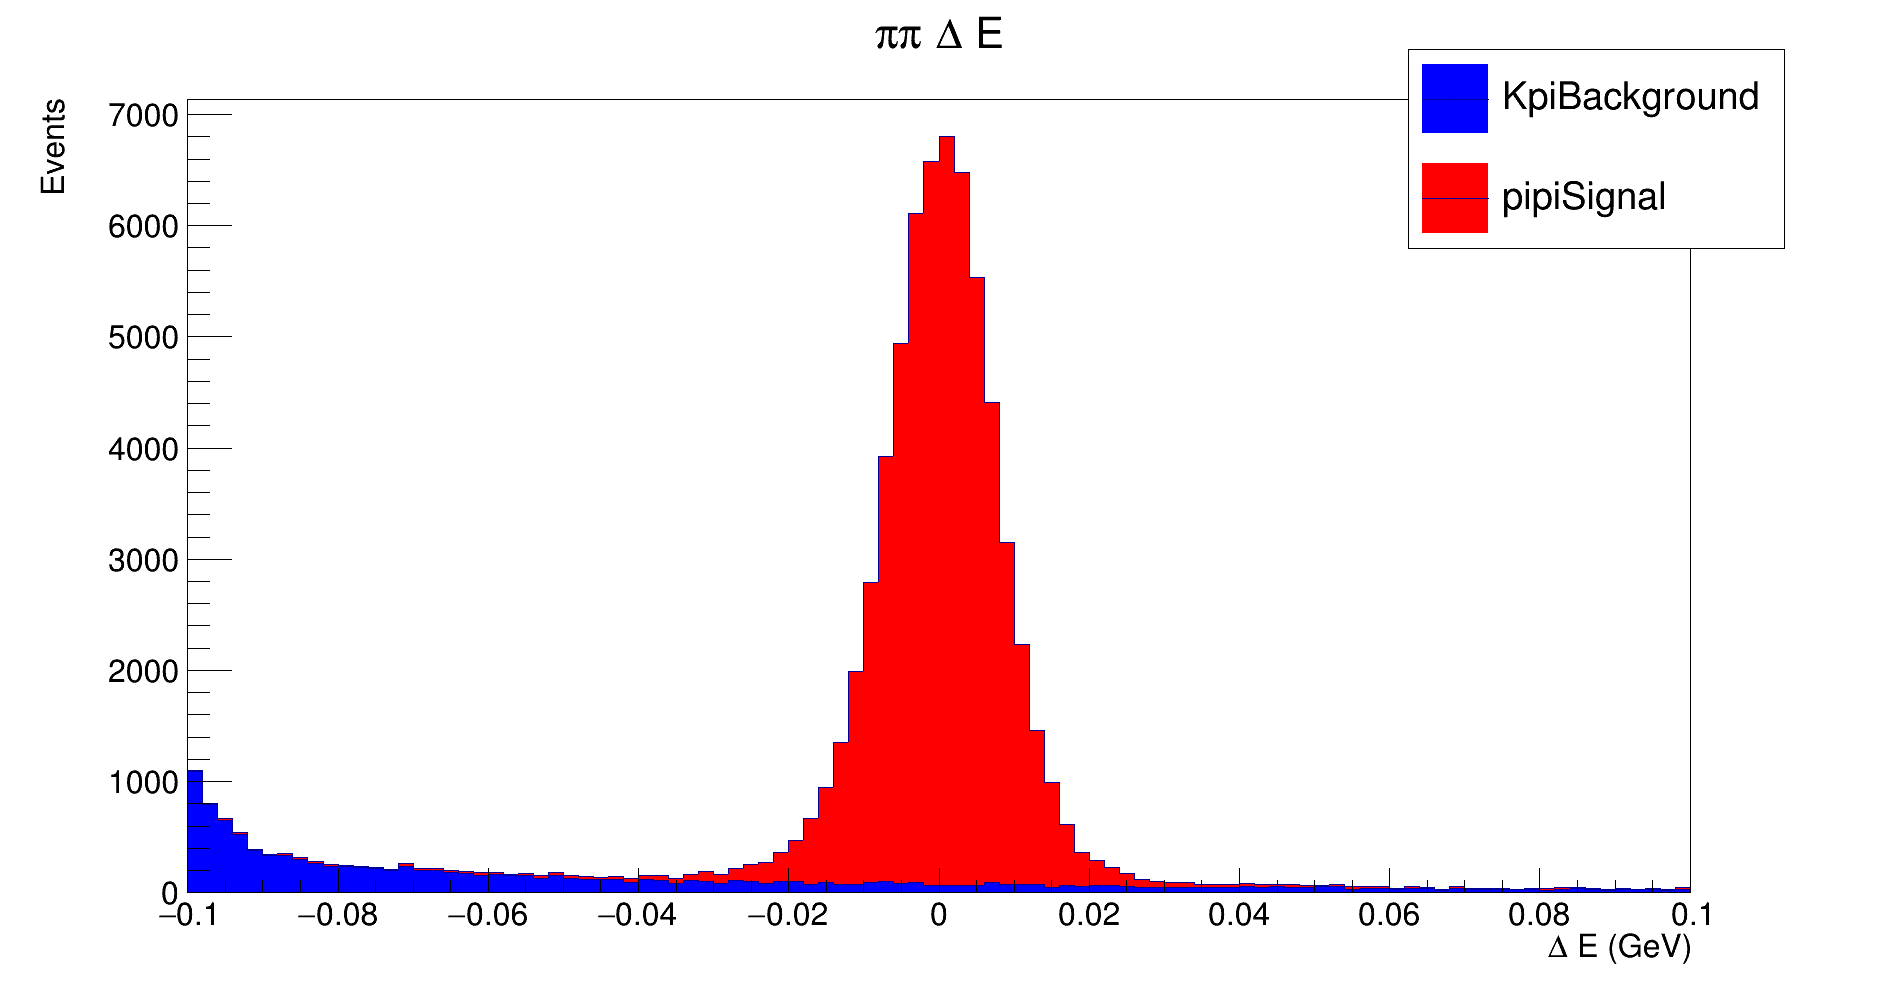
\includegraphics[width=0.8\textwidth]{pipiDeltaEBackground.png}
  \end{figure}
  Question: How to fit this?
\end{frame}

\end{document}
